%% use_cases.tex

\section{Use cases}

Now it is time to play  with geometry models and the geometry factory.
We will start  by a very simple case and will  introduce more and more
complexity progressively.

\subsection{A box in a virtual world}

We  want to achieve  the construction  of the  virtual setup  shown on
figure \ref{fig:mf:0}.   We have here  a simple top level  large green
box (the \emph{world}) with  given dimensions and auxiliary properties
(color,  material\dots).   This \emph{world}  box  contains a  single
smaller red  box with its  own geometry and auxiliary  properties. The
placement of the red box inside  the mother green box is determined by
the position  of the center  $O'$ of the  red box with respect  to the
center $O$  of the green box.   The orientation of the  red box inside
the mother green box can  be determined by the Euler angles associated
to  the rotation matrix  that transform  the ($0xyz$)  world reference
frame axis into the ($0'x'y'z'$) daughter frame axis.


\begin{figure}[h]
\begin{center}
\scalebox{0.75}{\input{\pdftextpath/fig_mf_0.pdftex_t}}
\end{center}
\caption{A very simple world.}\label{fig:mf:0}
\end{figure}

With  \texttt{geomtools}, the  easiest way  to construct  this virtual
geometry setup is to use two available geometry model classes :
\begin{itemize} 

\item  the \texttt{geomtools::simple\_world\_model} class  is designed
  to model a  top-level box with arbitrary dimensions.  It can contain
  one and  only one daughter  volume at any position  and orientation:
  the \TT{setup} volume.   This daughter volume can be  modeled by any
  other geometry model available at run-time in the library.

\item the  \texttt{geomtools::simple\_shaped\_model} class is designed
  to address very  usual cases : volume with a  simple shape like box,
  cylinder,  sphere\dots.  Optionally  it  can contain  some  daughters
  volumes.

\end{itemize}

Both            \texttt{geomtools::simple\_world\_model}           and
\texttt{geomtools::simple\_shaped\_model} are registered by default in
the \texttt{geomtools}' \emph{model factory}.

What we  need now is to  provide some configuration file  with all the
directives that reflect the  layout seen on figure \ref{fig:mf:0}. The
file will use by convention the \texttt{.geom} extension, note however
it  is  not  mandatory.  The  format  is  the  ASCII encoding  of  the
\texttt{datatools::utils::multi\_properties}  class. The  principle is
to provide one  section of properties per geometry  model described in
the setup. Here we will have two section : one for the top-level world
model, the  second for the daughter  box in it. Note  that blank lines
are ignored as  well as line starting with the  \# character. There is
an exception  with special meta-comments starting  with \verb+#@+ that
are        part        of        the       syntax        of        the
\texttt{datatools::utils::multi\_properties}        and       embedded
\texttt{datatools::utils::properties} objects.  This meta-comments are
\verb+#@description+ and \verb+#@config+ (see the example below).

We first  create a file named \TT{simple\_world\_1.geom}  and we write
its header as shown on sample \ref{sample:header:1}.

\begin{sample}
\VerbatimInput[frame=single,
numbers=left,
numbersep=2pt,
firstline=1,
lastline=3,
fontsize=\footnotesize,
showspaces=false]{\codingpath/simple_world_1.geom}
\caption{The header of the  \TT{simple\_world\_1.geom} file.}
\label{sample:header:1}
\end{sample}


\pn This meta information,  stored as meta-comments, inform the parser
for  the \\  \texttt{datatools::utils::multi\_properties}  object that
each section  will have  a main key  labeled with \verb+name+  and an
additional tag labeled \verb+type+.  The \emph{name} will be used as
the primary key to access  each geometry model from an internal look-up
table.   The \emph{type}  is a  character string  that  identifies the
unique  geometry model  class that  must  be used  to instantiate  the
corresponding geometry model and  its associated logical volume; it is
thus used by the internal model factory.

\pn Now we are done with the logistics of \emph{multi\_properties} and
\emph{factory} objects, we can describe  the two models we need.  Here
again there is an important constraint.  As the small red box is to be
inserted in the lard world green  box. The geometry model of the green
box will \emph{depend on} the existence  of the small red box.  On the
other side, in this hierarchy, the small red box does not need to know
anything about the large green box. In principle, we could have chosen
to put it in another  cylindrical purple universe.  So to reflect this
mother/daughter  dependency,   we  \textbf{must}  first   declare  the
geometry model  for the small red  box. Then only we  will provide the
definition of the model that will instantiate the green world.

\pn The  small red box  use a very  simple shape. More, as  a terminal
leaf of  the hierarchy, it contains  no daughter. This  simple case is
addressed  by  the   \texttt{simple\_shaped\_model}  provided  by  the
\texttt{geomtools} API.

\pn The file sample \ref{sample:section_srb:1} shows 
the section for the \emph{small red box}.

\begin{sample}[h]
\VerbatimInput[frame=single,
numbers=left,
numbersep=2pt,
firstline=10,
lastline=30,
fontsize=\footnotesize,
showspaces=false]{\codingpath/simple_world_1.geom}
\caption{The \emph{small red box}
  section of the  \TT{simple\_world\_1.geom} file.}
\label{sample:section_srb:1}
\end{sample}

\pn Note that the mandatory parameters are:
\begin{itemize}

\item \texttt{shape\_type}, \texttt{x}, \texttt{y}, \texttt{z} : for a
  full geometry description of the volume,

\item \texttt{material.ref}  for this  is a crucial  physical property
  for client application.\\ Remark:  this behavior should be change in
  the  future to support,  for debugging  purpose, a  default material
  when this property is missing in the file.
\end{itemize}

\pn       Visibility      parameters      (\texttt{visibility.hidden},
\texttt{visibility.color}) are  optional.  However, because  there are
used  by the  Gnuplot  based fast  visualization  program provided  in
\texttt{geomtools}, we recommend to use them. They will also be passed
to the GEANT4 Open-GL visualization driver.

\pn Believe it or not, these  few lines will generate all the software
machinery to  handle the  3D-box object, set  its dimension,  add some
properties in it, and allocate  the associated logical volume. This is
transparent to the  user. At the end of the  processing of these lines
by the geometry model factory, a new object named \TT{small\_red\_box}
is inserted  in a  dynamic internal database  for further  usage. This
object now just has to wait to be used by some other (mother) geometry
model. Be patient, the \emph{world} is coming !

\pn So  what about the \emph{world}  volume ? As  mentioned above, the
\texttt{geomtools::simple\_world\_model} has  been implemented in this
purpose : hosting a single 3D object in a boxed universe.

\pn  Let's   write  the  \emph{world}   section  !  The   file  sample
\ref{sample:section_world:1}  stores  the   directives  that  must  be
written \textbf{after} the \TT{small\_red\_box} section :
\begin{sample}
\VerbatimInput[frame=single,
numbers=left,
numbersep=2pt,
firstline=37,
lastline=88,
fontsize=\footnotesize,
showspaces=false]{\codingpath/simple_world_1.geom}
\caption{The \emph{world}
  section of the  \TT{simple\_world\_1.geom} file.}
\label{sample:section_world:1}
\end{sample}

\pn It can  be seen here that this model needs  more information to be
properly described.  Not only it requires the dimensions, material and
visibility parameters,  but it  also needs some  geometry informations
for the placement  of the setup volume it  contains. The configuration
properties are rather self explanatory.

\pn  The  C++   program  \ref{program:section_world:1}  illustrates  a
minimal  use   of  the  \texttt{geomtools::model\_factory}   class  to
construct  the   virtual  geometry  model  that   corresponds  to  the
directives  stored in the  \TT{simple\_world\_1.geom} file.   Once the
factory object has loaded the file and has been locked, the transcient
geometry hierarchy model is built and the program prints its structure
on the terminal.
  

\begin{program}[h]
\VerbatimInput[frame=single,
numbers=left,
numbersep=2pt,
firstline=1,
%%lastline=88,
fontsize=\footnotesize,
showspaces=false]{\codingpath/simple_world_1.cxx}
\caption{A program for the  construction of the virtual geometry setup
  described in the \TT{simple\_world\_1.geom} file.}
\label{program:section_world:1}
\end{program}


\pn The following  C++ program \ref{program:section_world:2} shows how
to pass the geometry hierarchy model built by the \emph{geometry model
  factory} to some special driver : a Gnuplot renderer (visualization)
and  a GDML  filter.  Figure  \ref{fig:mf:simple_world_1:a}  shows the
Gnuplot  based 3D-display originated  from the  program. We  have been
able  to   achieve  the   goal  in  figure   \label{fig:mf:0}.  Sample
\ref{sample:gdml:1}  shows  the contents  of  the  GDML  file that  is
generated by the GDML export driver object.


\begin{program}[hp]
\VerbatimInput[frame=single,
numbers=left,
numbersep=2pt,
firstline=1,
%%lastline=88,
fontsize=\footnotesize,
showspaces=false]{\codingpath/simple_world_2.cxx}
\caption{A  program  that  extends  the  functionnalities  of  program
  \ref{program:section_world:1} and  display a  simple 3D view  of the
  geometry. It produces  also a GDML file that  describes the geometry
  setup.}
\label{program:section_world:2}
\end{program}

\begin{figure}[h]
\begin{center}
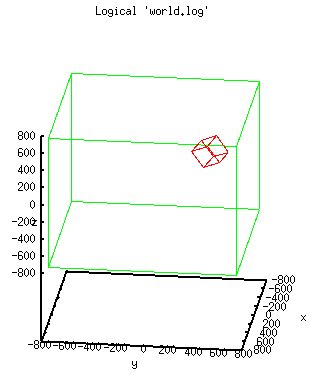
\includegraphics[width=0.75\linewidth]{\imagepath/simple_world_1.jpeg}
\end{center}
\caption{The Gnuplot  display of the simple  virtual world constructed
  from   the   file   \texttt{simple\_world\_1.geom}  built   by   the
  \ref{program:section_world:2}
  program.}\label{fig:mf:simple_world_1:a}
\end{figure}

\begin{sample}[hp]
\VerbatimInput[frame=single,
numbers=left,
numbersep=2pt,
firstline=1,
%%lastline=88,
fontsize=\tiny,
showspaces=false]{\codingpath/simple_world_2.gdml.save}
\caption{The     GDML     file     generated    by     the     program
  \ref{program:section_world:2}  from  the   setup  described  in  the
  \TT{simple\_world\_1.geom} file. Here a default list of materials is
  added by  the driver. In  a practical case,  a list of  materials is
  inserted by an external software agent.}
\label{sample:gdml:1}
\end{sample}

\clearpage

\subsection{A virtual world with two identical boxes in it}

We now address  a somewhat more complex setup :  we want two identical
small  red boxes to  be placed  within the  world volume  at different
(no overlapping) positions and orientations.

We  thus create  a new  \TT{setup\_2.geom} file  to describe  this new
geometry  layout.  Here  the description  of  the \TT{small\_red\_box}
geometry model is unchanged with regards to the previous setup (sample
\ref{sample:section_srb:1}). But now, as  we want to place two objects
within   the   \emph{world}  volume,   we   cannot   use  the   former
\texttt{geomtools::simple\_world\_model} geoemtry model.  In place, we
will  use a  \texttt{geomtools::simple\_shaped\_model}  model (with  a
\TT{box}  shape) but  we will  add some  directives in  the \TT{world}
section  to  inform  the  \emph{world}  volume that  it  contains  two
boxes.  To  achieve  this   we  use  special  directives  prefixed  by
\texttt{internal\_item}.

\pn The file  sample \ref{sample:section_world:2} shows the directives
that   must   be  written   in   the   \TT{world}   section  of   file
\TT{setup\_2.geom} in order to describe the new world volume :
\begin{sample}
\VerbatimInput[frame=single,
numbers=left,
numbersep=2pt,
firstline=37,
lastline=68,
fontsize=\footnotesize,
showspaces=false]{\codingpath/setup_2.geom}
\caption{The \emph{world}
  section of the  \TT{setup\_2.geom} file.}
\label{sample:section_world:2}
\end{sample}

Using   the   \texttt{setup\_construct\_and\_view.cxx}  program   (see
program  \ref{program:scav:0}),  we   obtain  the  display  in  figure
\ref{fig:setup_2:0}. 

\begin{program}[hp]
\VerbatimInput[frame=single,
numbers=left,
numbersep=2pt,
firstline=4,
fontsize=\footnotesize,
showspaces=false]{\codingpath/setup_construct_and_view.cxx}
\caption{The \texttt{setup\_construct\_and\_view.cxx} program.}
\label{program:scav:0}
\end{program}

\begin{figure}[h]
\begin{center}
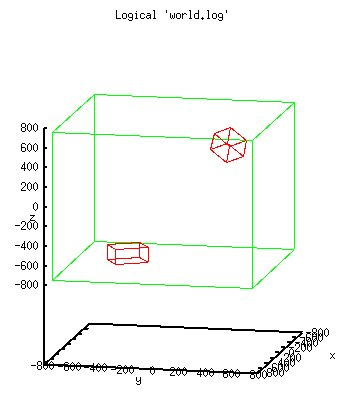
\includegraphics[width=0.75\linewidth]{\imagepath/setup_2.jpeg}
\end{center}
\caption{The Gnuplot  display of the  virtual world constructed
  from   the   file   \texttt{setup\_2.geom}  built   by   the
  \ref{program:scav:0} program.}\label{fig:setup_2:0}
\end{figure}


\clearpage

\subsection{A virtual world with several objects of different types\dots}

Adding more  boxes is trivial, we  just have to  extend the \TT{world}
section's   \texttt{internal\_item.labels}   list   of   labels   with
additional      names      and      provide     the      corresponding
\texttt{internal\_item.model.XXX}                                   and
\texttt{internal\_item.placement.XXX}  rules.  But we  can also  get a
mix  of different  kind of  objects as  daughters of  the \emph{world}
volume.  

In  a new  \TT{setup\_3.geom}  file, let's  introduce,  after the  
well known  \TT{small\_red\_box} section,  a new  geometry  model that
represents a  long blue cylinder.  This  is done with  the file sample
\ref{sample:setup_3:0} that shows the  parameters of a new section for
the cylindric object.

\begin{sample}[h]
\VerbatimInput[frame=single,
numbers=left,
numbersep=2pt,
firstline=26,
lastline=34,
fontsize=\footnotesize,
showspaces=false]{\codingpath/setup_3.geom}
\caption{The \emph{long blue cylinder}
  section of the  \TT{setup\_3.geom} file.}
\label{sample:setup_3:0}
\end{sample}

The \TT{world} section now writes like in sample \ref{sample:setup_3:1}.
\begin{sample}[h]
\VerbatimInput[frame=single,
numbers=left,
numbersep=2pt,
firstline=41,
lastline=60,
fontsize=\footnotesize,
showspaces=false]{\codingpath/setup_3.geom}
\caption{The \emph{world} section of the \TT{setup\_3.geom} file.}
\label{sample:setup_3:1}
\end{sample}

Now the \texttt{setup\_construct\_and\_view.cxx} program (program source 
\ref{program:scav:0}) displays the figure \ref{fig:setup_3:0}.
Easy isn't it ?

\begin{figure}[h]
\begin{center}
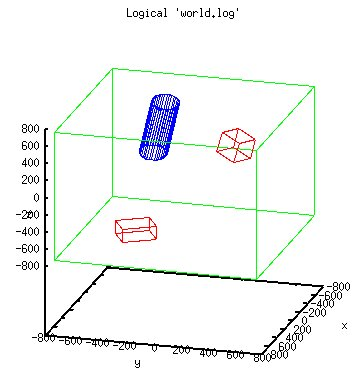
\includegraphics[width=0.75\linewidth]{\imagepath/setup_3.jpeg}
\end{center}
\caption{The Gnuplot  display of the  virtual world constructed
  from   the   file   \texttt{setup\_3.geom}  built   by   the
  \ref{program:scav:0} program.}\label{fig:setup_3:0}
\end{figure}

\clearpage

\subsection{A setup with more hierarchy levels}

This section describes a more complex setup. Now we will implement a
world volume that contains not only a long blue cylinder but also
a huge magenta cube that contains in turn three small red boxes
with arbitrary placements. 

File samples \ref{sample:setup_4:1} and \ref{sample:setup_4:2}
show the associated sections of a new file \TT{setup\_4.geom}.
The display of this three-level hierarchy setup can be sen on figure \ref{fig:setup_4:0}.

There is no limit to the number of levels we can handle with such mecanism.
The \texttt{internal\_item.XXX} rule can be used to nest more and more 
daughter volumes at higher depth.

\begin{sample}[h]
\VerbatimInput[frame=single,
numbers=left,
numbersep=2pt,
firstline=41,
lastline=58,
fontsize=\footnotesize,
showspaces=false]{\codingpath/setup_4.geom}
\caption{The \emph{huge magenta cube}
  section of the  \TT{setup\_4.geom} file.}
\label{sample:setup_4:1}
\end{sample}

\begin{sample}[h]
\VerbatimInput[frame=single,
numbers=left,
numbersep=2pt,
firstline=65,
lastline=82,
fontsize=\footnotesize,
showspaces=false]{\codingpath/setup_4.geom}
\caption{The \emph{world} section of the \TT{setup\_4.geom} file.}
\label{sample:setup_4:2}
\end{sample}

\begin{figure}[h]
\begin{center}
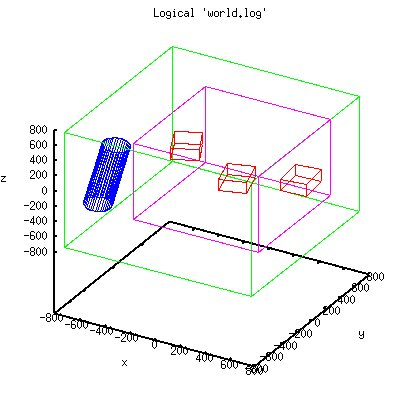
\includegraphics[width=0.75\linewidth]{\imagepath/setup_4.jpeg}
\end{center}
\caption{The Gnuplot  display of the  virtual world constructed
  from   the   file   \texttt{setup\_4.geom}.}\label{fig:setup_4:0}
\end{figure}

\clearpage

\subsection{Smart geometry models}

We have  seen in  the previous  section the basics  to build  a nested
geometry.  Up to now, we only  have placed some volumes in some mother
volumes  thanks to  the  \emph{internal item}  technique. However  the
placement of all this daughter  objects was arbitrary. We were obliged
to explicitely give the positions and rotation angles of each daughter
object with respect to the coordinate system of their mother volume.

In practical  situations, we often face  the case of  the placement of
objects -- in a mother volume -- following some symmetrical or regular
patterns. This  can be seen  on figure \ref{fig:smart:0}  with several
objects built from  the same model and placed  regularly along a given
symmetry axis.


\begin{figure}[h]
\begin{center}
\scalebox{0.75}{\input{\pdftextpath/fig_smart_0.pdftex_t}}
\end{center}
\caption{A mother volume with some replicated daughter volumes.}
\label{fig:smart:0}
\end{figure}

The \texttt{geomtools} library provides a few useful models that allow
to  automatically placed  some volumes  inside a  mother  volume using
special patterns :


\subsubsection{The \texttt{rotated\_boxed\_model} driver}

This geometry model enables to  create a wrapper model that operates a
rotation  on a given  box shaped  model. The  rotated daughter  box is
included  in a  mother box  of which  dimensions can  be automatically
computed if special rotation angles are used.

The sample  \ref{sample:rotated:0} shows the  syntax used to  define a
\texttt{rotated\_boxed\_model}  driver  using the  $Oz$  axis with  an
arbitrary  rotation  angle.  The  rotation  operates  on a  predefined
box-shape model. As the rotation operates on the $Oz$ axis, the height
of the mother volume equals the height of the daughter volume. However
the width (\texttt{x})  and depth (\texttt{y}) of the  mother box must
be provided by the user in such a way the mother box fully enclose the 
daughter volume.

Another  possibility is shown  with sample  \ref{sample:rotated:1}. In
this case a \emph{special} rotation angle around the $0x$ axis is used
(can be  0, 90, 180 or  270 $^{\circ}$).  The  mother volume's dimensions
are automatically computed so there  is no need to pass the transverse
dimensions \texttt{y} and \texttt{z}.

\begin{sample}[h]
\VerbatimInput[frame=single,
numbers=left,
numbersep=2pt,
firstline=26,
lastline=38,
fontsize=\footnotesize,
showspaces=false]{\codingpath/setup_5.geom}
\caption{The syntax for a \emph{rotated box model} section.}
\label{sample:rotated:0}
\end{sample}

\begin{sample}[h]
\VerbatimInput[frame=single,
numbers=left,
numbersep=2pt,
firstline=45,
lastline=54,
fontsize=\footnotesize,
showspaces=false]{\codingpath/setup_5.geom}
\caption{The  syntax for a  \emph{rotated box  model} using  a special
  angle.}
\label{sample:rotated:1}
\end{sample}

The  sample \ref{sample:rotated:2}  shows a  \emph{world}  volume that
contains three boxes  with two of them rotated  with these mechanisms.
The  box in  magenta materializes  the  mother volume  of the  central
rotated box (in red inside). The figure \label{fig:setup_5:0} displays
the setup.

\begin{sample}[h]
\VerbatimInput[frame=single,
numbers=left,
numbersep=2pt,
firstline=61,
lastline=78,
fontsize=\footnotesize,
showspaces=false]{\codingpath/setup_5.geom}
\caption{The section of the \emph{world} volume with rotated boxed models.}
\label{sample:rotated:2}
\end{sample}

\begin{figure}[h]
\begin{center}
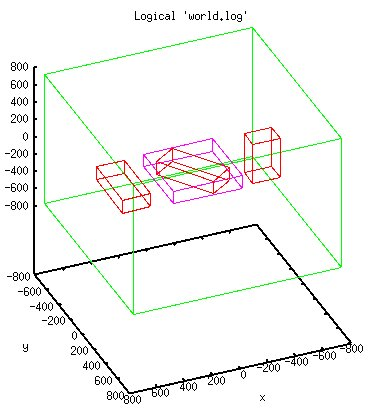
\includegraphics[width=0.75\linewidth]{\imagepath/setup_5.jpeg}
\end{center}
\caption{The Gnuplot  display of  the virtual world  with a  first non
  rotated box (left),  a box rotated by some  arbitrary angle (center)
  and a box rotated by some special angle (right).}
\label{fig:setup_5:0}
\end{figure}

\subsubsection{The \texttt{replicated\_boxed\_model} driver}

This geometry model enables to  build a box-shaped mother volumes that
contains  an arbitrary  numbers of  adjacent (no  space  between them)
daugther copies of  one unique box shaped geometry  model along one of
its main axis ($x$, $y$ or $z$).

The sample \ref{sample:replicated:0} shows the syntax used to define a
\texttt{replicated\_boxed\_model} driver using  the $Ox$ axis to place
4 copies  of a  box shape model.   The mother volume's  dimensions are
automatically computed.

The sample \ref{sample:replicated:1} replicate the above replicated
model on the $Oy$ axis. It results in a grid layout of boxex.

\begin{sample}[h]
\VerbatimInput[frame=single,
numbers=left,
numbersep=2pt,
firstline=26,
lastline=32,
fontsize=\footnotesize,
showspaces=false]{\codingpath/setup_6.geom}
\caption{The syntax for a \emph{replicated box model} section.}
\label{sample:replicated:0}
\end{sample}


\begin{sample}[h]
\VerbatimInput[frame=single,
numbers=left,
numbersep=2pt,
firstline=39,
lastline=45,
fontsize=\footnotesize,
showspaces=false]{\codingpath/setup_6.geom}
\caption{The  syntax for another  \emph{replicated box  model}.}
\label{sample:replicated:1}
\end{sample}

The  sample \ref{sample:replicated:2}  shows the  \emph{world}  volume that
contains this grid mother volume. The figure \label{fig:setup_6:0} displays
the setup.

\begin{sample}[h]
\VerbatimInput[frame=single,
numbers=left,
numbersep=2pt,
firstline=52,
lastline=69,
fontsize=\footnotesize,
showspaces=false]{\codingpath/setup_6.geom}
\caption{The section of the \emph{world} volume with replicated boxed models.}
\label{sample:replicated:2}
\end{sample}

\begin{figure}[h]
\begin{center}
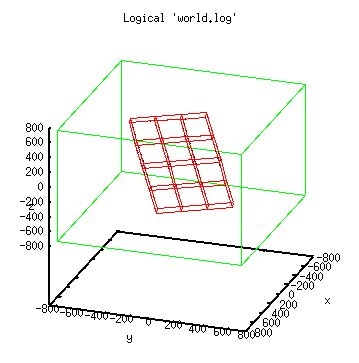
\includegraphics[width=0.75\linewidth]{\imagepath/setup_6.jpeg}
\end{center}
\caption{The Gnuplot  display of  the virtual world  with a  grid made
  from a two levels replicated model.}
\label{fig:setup_6:0}
\end{figure}

\subsubsection{The \texttt{surrounded\_boxed\_model} driver}

This model is used when one  wants to assemble objects on some part or
all of the faces of a central box shape model.

The sample \ref{sample:surrounded:0} shows the syntax used to define a
\texttt{surrounded\_boxed\_model} driver  with three different volumes
placed  on  three  faces  of  a  central  box.   The  mother  volume's
dimensions        are        automatically        computed.        The
figure \label{fig:setup_7:0} displays the setup.

Some  boolean options  are available  to  force the  centering of  the
assembly within the mother volume. There is one option per $x$, $y$ or
$z$               axis:               \texttt{surrounded.centered\_x},
\texttt{surrounded.centered\_y}  and  \texttt{surrounded.centered\_z}.
The \texttt{surrounded.bottom\_model}, \texttt{surrounded.top\_model},
\texttt{surrounded.back\_model},      \texttt{surrounded.front\_model},
\texttt{surrounded.left\_model}  and  \texttt{surrounded.right\_model}
parameters are all  optional and allow to specify the  name of a model
to be assembled on the corresponding face of the central model.

\begin{sample}[h]
\VerbatimInput[frame=single,
numbers=left,
numbersep=2pt,
firstline=69,
lastline=80,
fontsize=\footnotesize,
showspaces=false]{\codingpath/setup_7.geom}
\caption{The syntax for a \emph{surrounded box model} section.}
\label{sample:surrounded:0}
\end{sample}


\begin{figure}[h]
\begin{center}
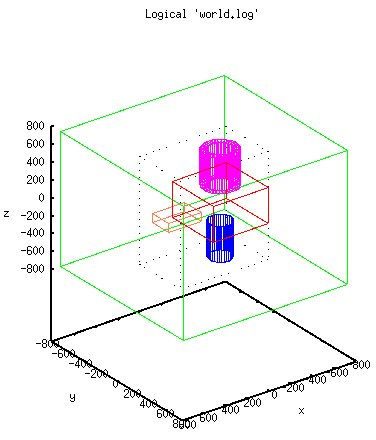
\includegraphics[width=0.75\linewidth]{\imagepath/setup_7.jpeg}
\end{center}
\caption{The  Gnuplot  display  of   the  virtual  world  with  a  box
  surrounded by other volumes and wrapped in its mother envelope.}
\label{fig:setup_7:0}
\end{figure}


\subsubsection{The \texttt{stacked\_model} driver}

The \texttt{stacked\_model} driver is responsible to stack several objects
along an arbitrary axis ($x$, $y$ or $z$). A mother volume is automatically 
computed to enclose the full set of stacked daughter volumes. Stacked objects
must fulfill the \emph{stackable object} interface; boxes, cylinders, 
tubes as well as other basic shapes do. 

The sample  \ref{sample:stacked:0} shows the  syntax used to  define a
\texttt{stacked\_model}  driver  with  four different  volumes  placed
along the $0z$ axis.  The mother volume's dimensions are automatically
computed.  The figure \label{fig:setup_8:0} displays the setup.

The  dimensions  of  the  mother  box  can  be  enforced  rather  than
automatically  computed through  the optional  \texttt{x}, \texttt{y},
\texttt{z} real parameters  (associated with the \texttt{length\_unit}
string property).  In this case,  the dimensions must ensure  that the
daughter volumes are fully contained in the mother box.

\begin{sample}[h]
\VerbatimInput[frame=single,
numbers=left,
numbersep=2pt,
firstline=69,
lastline=80,
fontsize=\footnotesize,
showspaces=false]{\codingpath/setup_8.geom}
\caption{The syntax for a \emph{stacked model} section.}
\label{sample:stacked:0}
\end{sample}

\begin{figure}[h]
\begin{center}
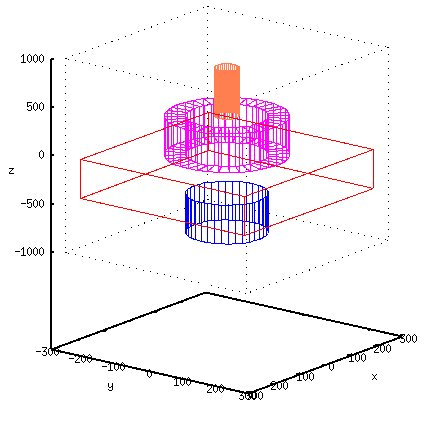
\includegraphics[width=0.75\linewidth]{\imagepath/setup_8.jpeg}
\end{center}
\caption{The Gnuplot display of the virtual world with a stack of four
  different  volumes along  the $z$  axis  and wrapped  in its  mother
  envelope.}
\label{fig:setup_8:0}
\end{figure}


Some additional rules can be  added to allow complex stacking as shown
on figure  \ref{fig:stacked:1}. This case  can occur when  some volume
has some  concave shape along  the stacking axis. A  stacked neighbour
convex volume  with smaller dimension(s) can  interpenetrate (at least
partially)  the  concave region  of  the  former  shape.  By  default,
\emph{stackable objects}  has some default bounds  (large purple arrow
on  the  figure)  that  allow  only  stacking  algorithm  to  assemble
neighbour  volume by  such bounds.   With  the \texttt{stacked\_model}
driver, it is  possible to redefine new bounds for  a volume along the
stacking  axis and  thus  allow some  penetrating  placement of  other
volumes.   For  each  stacked  model,   it  is  possible  to  use  the
\texttt{stacked.limit\_min\_X} and \texttt{stacked.limit\_max\_X} real
rules. As seen of figure  \ref{fig:stacked:2}, these bounds can be set
arbitrarily and  the choice  depends on what  layout the user  want to
achieve. The sample \ref{sample:stacked:1}  shows a typical syntax for
these options and figure  \label{fig:setup_9:0} shows the setup.

\begin{figure}[h]
\begin{center}
\scalebox{0.75}{\input{\pdftextpath/fig_stacked_1.pdftex_t}}
\end{center}
\caption{Special stacking with interpenetrating volumes.}\label{fig:stacked:1}
\end{figure}

\begin{figure}[h]
\begin{center}
\scalebox{0.75}{\input{\pdftextpath/fig_stacked_2.pdftex_t}}
\end{center}
\caption{Setting new  stacking bounds to a volume.  Purple arrows show
  the new  bounds applied to  the volume. The green  spheres indicates
  the     extreme    positions     allowed     by    these     stacking
  informations.}\label{fig:stacked:2}
\end{figure}

\begin{sample}[h]
\VerbatimInput[frame=single,
numbers=left,
numbersep=2pt,
firstline=68,
lastline=85,
fontsize=\footnotesize,
showspaces=false]{\codingpath/setup_9.geom}
\caption{The syntax for a \emph{stacked model} section with penetrating volumes.}
\label{sample:stacked:1}
\end{sample}

\begin{figure}[h]
\begin{center}
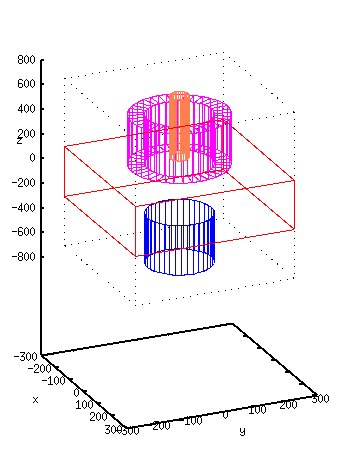
\includegraphics[width=0.75\linewidth]{\imagepath/setup_9.jpeg}
\end{center}
\caption{The Gnuplot display of stacked volumes with penetrating placement.}
\label{fig:setup_9:0}
\end{figure}

%% end of use_cases.tex
